\def \Subject {گام چهارم}

% \def \Session {2}
% \setcounter{chapter}{\Session}

\section{\Subject}

\begin{itemize}
\item 
{
ابتدا هیستوگرام 
\(y\)
را رسم می کنیم.
  \begin{figure}[h!]
    \centering
    \makebox[\textwidth][c]{%
    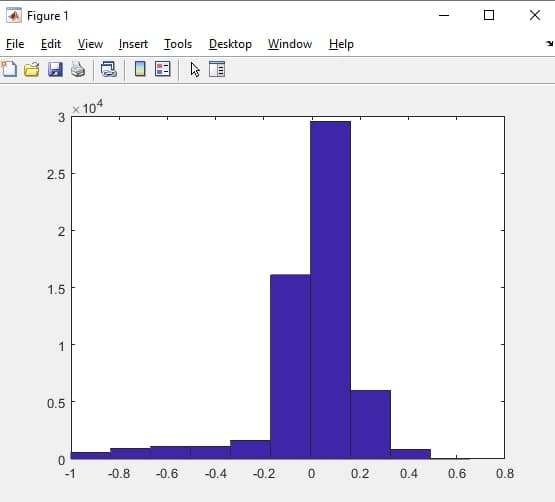
\includegraphics[height=0.5\textheight,width=0.7\textwidth]{images/hist_y.jpg}%
    }
\end{figure}
}
\item  
{
سپس با استفاده از اطلاعاتی که از هیستوگرام استخراج می کنیم، انتروپی این منبع را بدست می آوریم.

\begin{latin}
    \inputminted[frame=none]{csharp}{s_4_1.cs}
\end{latin}

خروجی کد بالا
\(Hx = 1.9656\)
شد.
}
\item 
{
طبق قضیه اول شانون 
\(n\)
متغیر تصادفی با انتروپی 
\(H(x)\)
را می توان به 
\(nH(x)\)
بیت بدون از دست دادن اطلاعات فشرده ساخت.

\begin{latin}
    \inputminted[frame=none]{csharp}{s_4_2.cs}
\end{latin}



خروجی کد بالا
\(e = 1.1363e+05\)
شد. یعنی این فایل را تا 
\(113\)
کیلوبایت می توان فشرده کرد.
}
\item{
به نظر شما نتیجه بدست آمده معقول است؟ اگر نیست چرا؟ تحقیق کنید و ببینید آیا می توان به مرزهای
واقعی تری برای فشرده سازی دست یافت؟
نه معقول نیست، زیرا سمبل ها مستقل در نظر گرفته شدند ولی در واقعیت اینگونه نیست. همانند مثال کلمات، بعضی کلمات در کنار هم ظاهر نمی شوند یا برعکس و یا احتمال رخداد یک کلمه خیلی بیشتر از بعضی کلمات دیگر باشد. 
}
\end{itemize}



